% \begin{tikzpicture}
%     \tikzstyle{every node}=[font=\scriptsize]
%     \definecolor{tabblue}{RGB}{31, 119, 180}
\definecolor{taborange}{RGB}{255, 127, 14}
\definecolor{tabgreen}{RGB}{44, 160, 44}
\definecolor{tabred}{RGB}{214, 39, 40}
\definecolor{tabpurple}{RGB}{148, 103, 189}
\definecolor{tabbrown}{RGB}{140, 86, 75}
\definecolor{tabpink}{RGB}{227, 119, 194}
\definecolor{tabgray}{RGB}{127, 127, 127}
\definecolor{tabolive}{RGB}{188, 189, 34}
\definecolor{tabcyan}{RGB}{23, 190, 207}
\definecolor{ForestGreen}{RGB}{34, 139, 34}
%     \begin{axis}[%
%     hide axis,
%     xmin=10,
%     xmax=50,
%     ymin=0,
%     ymax=0.1,
%     legend style={
%         draw=white!15!black,
%         legend cell align=left,
%         legend columns=3,
%         legend style={
%             draw=none,
%             column sep=1ex,
%             line width=1pt,
%         }
%     },
%     ]

%     \addlegendimage{
%         line legend,
%         tabblue,
%         thick,
%         mark=square*,
%         mark options={line width=1.5pt, rotate=45}
%     }
%     \addlegendentry{\textbf{PEACH Encoder} (Ours)}
%     \addlegendimage{line legend, tabgreen, thick, mark=triangle*, mark options={line width=1.5pt, rotate=0}}
%     \addlegendentry{GNN Encoder}
%     \addlegendimage{
%         line legend,
%         taborange,
%         thick,
%         mark=square*,
%         mark options={line width=1.5pt, rotate=0}
%     }
%     \addlegendentry{PSTNet Encoder}
%     % New Line
%     % \addlegendimage{empty legend}
%     % \addlegendentry{}

%     \addlegendimage{line legend, tabolive, thick, mark=x, mark size=3pt, mark options={line width=1pt}}
%     \addlegendentry{Oracle Encoder}
%     \addlegendimage{line legend, tabcyan, thick, mark=+, mark size=2.5pt, mark options={line width=2pt}}
%     \addlegendentry{MaNGO Mesh Encoder}
%     \addlegendimage{line legend, tabgray, thick, mark=*}
%     \addlegendentry{No Context Encoder}    
%     \end{axis}
% \end{tikzpicture}

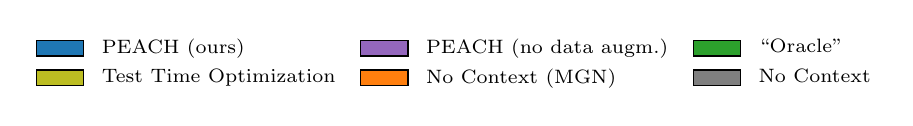
\begin{tikzpicture}
    \tikzstyle{every node}=[font=\scriptsize]
    \definecolor{tabblue}{RGB}{31, 119, 180}
\definecolor{taborange}{RGB}{255, 127, 14}
\definecolor{tabgreen}{RGB}{44, 160, 44}
\definecolor{tabred}{RGB}{214, 39, 40}
\definecolor{tabpurple}{RGB}{148, 103, 189}
\definecolor{tabbrown}{RGB}{140, 86, 75}
\definecolor{tabpink}{RGB}{227, 119, 194}
\definecolor{tabgray}{RGB}{127, 127, 127}
\definecolor{tabolive}{RGB}{188, 189, 34}
\definecolor{tabcyan}{RGB}{23, 190, 207}
\definecolor{ForestGreen}{RGB}{34, 139, 34}

    \begin{axis}[%
        hide axis,
        xmin=10,
        xmax=50,
        ymin=0,
        ymax=0.1,
        legend style={
            draw=none,
            legend cell align=left,
            legend columns=3,
            /tikz/every odd column/.append style={column sep=1ex},
            /tikz/every even column/.append style={column sep=1.6ex},
        }
    ]

    % --- Bar-style legend entries ---
    \addlegendimage{area legend, fill=tabblue}
    \addlegendentry{PEACH (ours)}

    \addlegendimage{area legend, fill=tabpurple}
    \addlegendentry{PEACH (no data augm.)}

    \addlegendimage{area legend, fill=tabgreen}
    \addlegendentry{``Oracle''}


    \addlegendimage{area legend, fill=tabolive}
    \addlegendentry{Test Time Optimization}

    
    \addlegendimage{area legend, fill=taborange}
    \addlegendentry{No Context (MGN)}

    \addlegendimage{area legend, fill=tabgray}
    \addlegendentry{No Context}
    \end{axis}
\end{tikzpicture}